\documentclass[]{article}

%opening
\title{Piecewise Linear Programming with PULP}
\author{Tom van der Hoeven}
\usepackage{tikz, amsmath}

\DeclareMathOperator*{\minimize}{minimize}
\usepackage{amsfonts}% to get the \mathbb alphabet
\newcommand{\field}[1]{\mathbb{#1}}
\newcommand{\R}{\field{R}}
\newcommand{\streepje}{+(0,0.2) -- +(0,-0.2)}
\newcommand{\fx}[3]{\draw (#1,#2) node(fx#3){$f_{#3}(x_{#3})$}}
\newcommand{\for}[0]{\text{ for }}
\newcommand{\en}[0]{\text{ and }}
\newcommand{\so}[0]{\text{ so }}
\newcommand{\cost}[0]{\text{cost}}
\newcommand{\plf}[0]{\text{plf}}
\newcommand{\SP}[0]{\text{SP}}
\newcommand{\force}[0]{\text{force}}
\newcommand{\Dual}[0]{\text{Dual}}
\setlength\parindent{0pt}
\begin{document}

\maketitle

\begin{abstract} \noindent
Convex piecewise linear programming is a small and useful extension to linear programming.
However not all linear programming packages have this extension.
By introducing extra variables in an organized way an LP package can be used for PLP purposes.
This article describes a set of Python modules wich allow easy formulation
of a PLP problem with variables and equations.
The CBC solver is accessed via the PULP package.
\end{abstract}

\section{Introduction}
The convex piecewise linear prgramming problem is
\[ \begin{cases}
         \minimize          & C(x) \quad \quad x \in \R^n \\
         \text{where}       & C(x) = \sum_{i=1}^{n} \text{plf}_i(x_i) \\
         \text{subject to}  & Ax=b \quad \quad b \in \R^m
   \end{cases} \]
Here follow a few examples of piecewise linear functions (plf).
A plf can be defined over $\R$ or over an interval. In case a plf has only one slope,
we just have a linear problem. A plf consist of breakpoints and slopes. 
\[ \text{plf} = ( s, p, s, p)\]

\newcommand{\fxy}[1]
{
  \draw (0,0)  (5,0) node(xline) {} ;
  \foreach \i [evaluate={\pl=int(\i-1);\pr=int(\i+1);}] in #1 % punten
  \ifodd \i %punten
       { \draw[gray,very thin] (p\i) -- (p\i |- xline) node[black,below] {$p_\i$} ;}
     \else %slopes
       { \draw (p\pl) -- (p\pr) node[sloped, midway, above] {$s_\i$} ;}
     \fi
;}
  \begin{tikzpicture}[x=23,y=25]
     \coordinate (p-1) at (0,4);
     \coordinate (p1) at (1,2);
     \coordinate (p3) at (2,1);
     \coordinate (p5) at (3.5,1.5);
     \coordinate (p7) at (5,4);
     \fxy{{0,...,6}}
  \end{tikzpicture}
%
  \begin{tikzpicture}[x=23,y=25]
     \coordinate (p1) at (1,1);
     \coordinate (p3) at (3,2);
     \coordinate (p5) at (5,5);
     \fxy{{1,...,4}}
  \end{tikzpicture}
%
  \begin{tikzpicture}[x=23,y=25]
     \coordinate (p1) at (1,1);
     \coordinate (p3) at (4,2);
     \fxy{{1, 2, 3}}
  \end{tikzpicture}

\section{Soft boundaries}
If an LP problem is infeasable it is often hard to find what is wrong.
Instead of using hard boundaries one can use plf's with the original boundaries as points
and left and right a penalty.
We call this soft boundaries and if the solution is outside the soft boundaries
we have a soft violation.
The values of the penalties must be chosen such that the interpretation of a soft violation is easy.
Eventualy some boundaries can be applied as hard bondaries.
In that case one must make sure that there is a feasible solution within the hard boundaries.

\section{Example}
\newcommand{\ov}[1]{\overline{#1}}
\newcommand{\un}[1]{\underline{#1}}
\newcommand{\ster}[1]{\draw (#1) +(0:-0.2)--+( 0:0.2) +(60:-0.2)--+( 60:0.2) +( -60:-0.2)--+(-60:0.2);}
\newcommand{\voeding}[2]{
%  \ster{#1-1.5,0}
  \ster{#2:#1-1.5}
%  \draw [->] (#1-1.5,0) +(0.1,0) -- +(1.4,0);
  \draw [<-] (#1,0) + (#2:-0.1) -- +(#2:-1.4);
}
\newcommand{\punt}[1]{ \fill (#1) circle[radius= 0.1,fill = red]; }          
\newcommand{\leiding}[2]{
   \punt{#1,0}
   \draw (#1,0) +(0.1,0) -- (#2-0.1,0);
   \punt{#2,0}
}
\newcommand{\compressor}[1]{
   \draw (#1+1,0) +(-0.9,0)--+(-0.5,0) +(0,0)circle[radius=0.5] 
   +(120:0.5)--+(30:0.5) +(-120:0.5)--+(-30:0.5)
   +(0.5,0)--+(0.9,0);
}
\newcommand{\reduceer}[1]{
   \draw (#1+1,0) +(-0.9,0)--+(-0.5,0)
    + (0.5,0.5)--+(-0.5,0.5)--+(-0.5,-0.5)--+(0.5,-0.5)--+ (0.5,0.5)
   +(0.5,0)--+(0.9,0);
   \draw[fill] (#1+1.5,0) -- +(-1,0.5) --+(-1,-0.5);
}
%\newcommand{\afname}[1]{ \draw [->] (#1+0.1,0) --(#1+1.4,0); }
\newcommand{\afname}[2]{ \draw [->] (#1,0) +(#2:0.1) -- +(#2:1.4); }

Consider a pipe between node A and B. 
The maximum pressure is 70 bar and the minimum contractual pressure is 40 bar.
Pressure cannot go below zero bar.
The contractual flow $Q = 400$.
The pipe equation $P_A - P_B = 0.1 Q$.
With $Q = 400$ it can be calculated that $P_A - P_B = 40$,
while the maximum pressure drop is 30 bar.
So this problem is infeasible, when we apply the constraints and equate the flow to 400.
   \begin{center}
      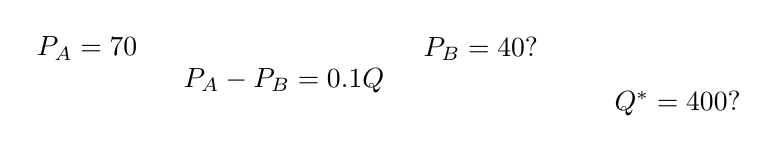
\begin{tikzpicture}[line width=1.0]
          \voeding{0}{0}  \leiding{0}{5} \afname{5}{0}
          \draw (0,0.7) node {$\ov{P}_A=70$} +(5,0) node {$\un{P}_B=40$?} ;
          %\draw (180:1.7) node[left,align=left] {cheap hot gas};
          %\draw (2.5,0.5) node {$c$} ;
          \draw (7.5,0) node{$Q^*= 400$?};
          \draw (2.5,0) node[above]{$P_A - P_B = 0.1 Q$};
      \end{tikzpicture}
%      \caption{Simulation based on solving equations}
      \label{cse}
   \end{center}
In this example there is always a solution if the pressures are between 0 and 70 bar,
and the flow is between 0 and 400.
So these values can be used as hard boundaries.
A soft boundary is on 40 bar, so there is a penalty of 1e5 below 40 bar.
If the pressures are between 40 and 70 we like the result to be as hight as possible,
so below 70 bar we put a small penalty of 0.01.
Al together for the pressures
\[ (p, s, p, s, p) = (0 ~~,~~ -1e5 ~~,~~ 40 ~~,~~ -0.01 ~~,~~ 70)\]
Lower and upper flow bound are 0 and 400, but the value 400 is very much wanted.
Below 400 we put a penalty of 1e3.
The resulting plf
\[ (p, s, p) = (0~~,~~ -1e3~~,~~ 400)\]
%
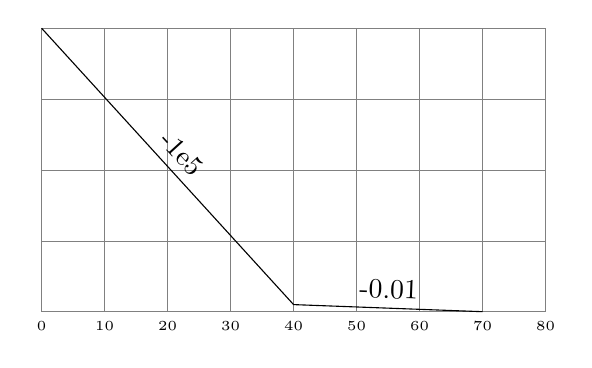
\begin{tikzpicture}[xshift=-3mm,x=0.08cm,y=0.9cm]
   \draw[gray,very thin, xstep = 10,ystep = 1] (0,0) grid(80,4);
   \draw (0,4) -- (40,0.1) node [sloped, midway, above] {-1e5}
               -- (70,0  ) node [sloped, midway, above] {-0.01} ;
   \foreach \x in {0,10,...,80} \draw { (\x,-0.2) node{\tiny{$\x$}}  } ;
\end{tikzpicture}
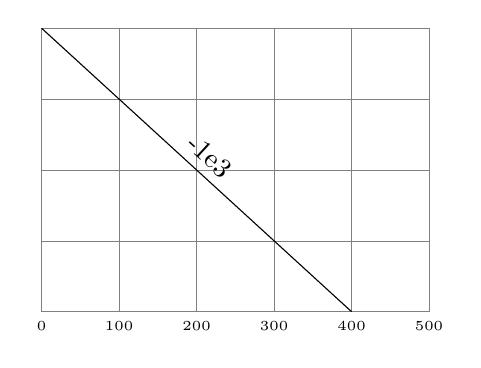
\begin{tikzpicture}[xshift=-3mm,x=0.28,y=0.9cm]
   \draw[gray,very thin, xstep = 100,ystep = 1] (0,0) grid(500,4);
   \draw (0,4) -- (400,0) node [sloped,midway,above] {-1e3} ;
   \foreach \x in {0,100,...,500} \draw { (\x,-0.2) node{\tiny{$\x$}}  } ;
\end{tikzpicture}

\begin{verbatim}
from plpcom import plpinit, plpvar, plpeq, plpexit, plpresults

plpinit()

PA = plpvar('pa',[None, 0, -1e5, 40, -0.01 , 70] )
PB = plpvar('pb',[None, 0, -1e5, 40, -0.01 , 70] )
Q  = plpvar('q' ,[None, 0, -1e3, 400] )

Epipe = plpeq('epi', [(1,PA), (-1,PB), (-0.1,Q)] )

plpexit(1)

print '               PA          PB           Q'
print 'x     {:11.2f} {:11.2f} {:11.2f} '.format(PA.x, PB.x, Q.x)
print 'force {:11.2f} {:11.2f} {:11.2f} '.format(PA.force, PB.force, Q.force)
\end{verbatim}
The result is 
\begin{verbatim}
               PA          PB           Q
x           70.00       40.00      300.00 
force    10000.00   -10000.00    -1000.00 
\end{verbatim}
The flow is not on target, but as hight as possible.
There is a positive force (10000) on pa (70) and a negative force (-10000) on pb (40).
This means that a larger maximum pressure or a lower minimum pressure
will give rise to a larger flow.
In this example the soft violation is on flow.
If the flow panalty is changed from 1e3 to 1e6 the violation will be on the soft pressure boundary.
\begin{verbatim}
Q.plf = [None, 0, -1e6, 400]
\end{verbatim}
The result is PA = 70, PB = 30 and Q = 400.

Another way to reach the same goal is to lessen the pressure penalty on PB.
The penalty must be lower than the force on PB from the first example, $9900 < 10000$.
\begin{verbatim}
PB.plf = [None, 0, -9900, 40, -0.01 , 70]
\end{verbatim}
Suppose that you want a flow of 800
\begin{verbatim}
Q.plf = [None, 0, -1e6, 800]
\end{verbatim}
Only a flow of 700 is reached because the pressure cannnot go below 0.

In this example the soft violations can easy be interpreted.
This holds for larger complicated networks as well.

\section{Reference}

\subsection{class plpvar}
The class variable plpvar.varis is a list of plpvar objects.
For instance plpvar.varis = [PA, PB, Q]
An object from the class plpvar has the following attributes:
\begin{center}
\begin{tabular}{|l|l|l|l|}\hline
  attribute & type     & in/res & description \\ \hline \hline
  name      & string   & input  & name \\ \hline
  plf       & list of scalars   & input  & plf  \\ \hline
  x         & scalar   & result & x value\\ \hline
  force     & scalar   & result & indirect derivative\\ \hline
  ix        & integer  & result & index in plf\\ \hline
  plfcost   & scalar   & result & plf(x)\\ \hline
\end{tabular}
\end{center}
A variables is instantiated in one out of three forms\\
A = plpvar('presa') \\
A = plpvar('presa', 3) \\
A = plpvar('presa', plf)\\
The name 'presa' is used by the LP solver and can be found in the results.
Without a second argument there is only one slope with $s = 0$.
If the second argument is a scalar we have one slope with $s = 3$.
If the second argument is a piecewise linear function we have plfcost(x) = plf(x)
A plf can always be changed after instantiatian of the variable, 
for instance A.plf = [None, 0, -1e6, 400]

\subsubsection{Piecewise linear function}
A piecewise linear function is described by points (x-values) and slopes. Examples:
\[ (p)~~,~~(s)~~,~~(p,s)~~,~~(s,p)~~,~~(p_1,s,p_2)~~,~~(s_1,p,s_2)
       ~~,~~(p_1,s_1,p_2,s_2)~~,~~\text{etcetera}\]
In the list representation an even index refers to a slope and an odd index refers to a point.
If a plf starts with a point the first member is None. So
\[ [None,p]~~,~~[s]~~,~~[None,p,s]~~,~~[s,p]
       ~~,~~[None,p_1,s,p_2]~~,~~[s_1,p,s_2]~~,~~\text{etcetera}\]
The list of points must be monotone increasing.
The list of slopes must be monotone increasing.
The lenght of the list is not limited.

Apart from a constant a plf is well defined.
A value $x_o$ can be choosen for which plf$(x_o)=0$.
If the plf has no points $x_o=0$ else one can choose
\begin{itemize}
\setlength\itemsep{-1mm}
  \item if $0 \in D$(plf) then $x_o=0$ else $x_o=x_k$ for the lowest value of $|x_k|$
  \item $x_o=x_k$ where $x_k$ minimize plf
\end{itemize}

\subsection{class plpeq}
The class variable plpeq.eqs is a list of plpeq objects.
For instance plpeq.eqs = [Epipe].
An object from the class plpeq has the following attributes:
\begin{center}
\begin{tabular}{|l|l|l|l|}\hline
  attribute & type     & in/res & description \\ \hline \hline
  naam    & string   & input  & name \\ \hline
  coefvar & list of tuples and scalars    & input  & plf  \\ \hline
  x       & scalar   & result 0 & x value\\ \hline
  force   & scalar   & result & indirect derivative\\ \hline
  ix      & integer  & result 1 &\\ \hline
\end{tabular}
\end{center}
An equation is instantiated by E = plpeq('eqa',coefvar)\\
E can be used for later reference and the name of the equation is 'eqa'\\
coefvar is a list of tuples and one or more scalars.
So if A = plpvar('x') and B = plpvar('y') and the equation is 6x - 3y = 7 ,\\
we get coefvar = [(6,A), (-3,B), -7]

\subsection{procedure plpinit}
The procedure plpinit set plpvar.varis = [ ] and plpeq.eqs = [ ]

\subsection{procedure plpexit}
The procedure plpexit transforms the plp variables to lp variables in PULP.
It executes the CBC solver and calculates the plp results.
%\newpage
\subsection{procedure plpresults}
The results can be listed by using plpresults().
For each variable plpresults() shows  the attibutes x, force, ix and plfcost.
\begin{verbatim}
{'maxnumber': 1000000, 'dosort': False, 'equat': False, 'minvalue': 0.0}
name                         x        force ix         cost    low-point
pa                       70.00     10000.00  5         0.00
pb                       40.00    -10000.00  3         0.30
aq                      300.00     -1000.00  2    100000.00       400.00
\end{verbatim}
If the solution is on a slope 
\begin{itemize}
\setlength\itemsep{-1mm}
 \item index ix is even
 \item the force is the slope value
 \item the low-point is the point with the lowest cost adjacent to the slope
 \end{itemize}
If the solution is on a point
\begin{itemize}
\setlength\itemsep{-1mm}
 \item index ix is odd 
 \item force is the (negative) shadow price
 \item slope-left $<$ force $<$ slope right
 \item if force $>$ 0 a higher value of the point is desirable
 \item if force $<$ 0 a lower value of the point is desirable
\end{itemize}

In case of soft voilation the lower point shows the soft constraint.
Normaly the results are obtained by referring to the attributes
of the variable object like PA.x or PA.force.
The procedure plpresults is used to get the variables with the largest cost or the largest force.
\begin{center}
\begin{tabular}{|l|l|l|l|}\hline
  keyword   & type    & description                    \\ \hline \hline
            & 'force' & sort on decreasing force       \\ \hline
  dosort    & 'cost'  & sort on decreasing cost        \\ \hline
            & 'name'  & sort on name                   \\ \hline
  maxnumber & integer & max number of results          \\ \hline
  minvalue  & real    & minimum value of force or cost \\ \hline
  equat     & boolean & show force on equations        \\ \hline
\end{tabular}
\end{center}

If there are soft violations, there is tention in the system.
Now plpresults(dosort = 'force', maxnumber = 30, minvalue = 1e4)
gives you maximum 30 results ordered on force, where force greater than 1e4.


\subsection{Adding plf's}
Sometimes a variable has cost or is bounded from two perspectives. In that case it is usefull to be able to add two plf's. Roughly speaking the points of the sum is a superset and the slopes are added.
sumplf = addplf(plf1, plf2)

\newpage
\section{Mathematics}
\subsection{Slope variables}
For each slope of a plf there has to be a lp variable.
Let $s$ be the index of a slope.
Let $c$ be the index of the central slope which has the minimal absolute value.
For plp variable $X$ Define the lp variable $X_c$ such that
\[ lb \le X_c \le ub \en \cost_{X_c} = \plf(c) X_k - \plf(c) x_o\]
For each other slope $s$ define a positive variable $X_s$ with
\begin{align*}
 \for s < c : X_s \ge 0 \en  X_s \ge -X_c + \plf(s+1) \en \cost_{Xs} = (\plf(s+2)-\plf(s) X_s \\
 \for s > c : X_s \ge 0 \en  X_s \ge +X_c - \plf(s-1) \en \cost_{Xs} = (\plf(s)-\plf(i-2) X_s
\end{align*}
\begin{center}
  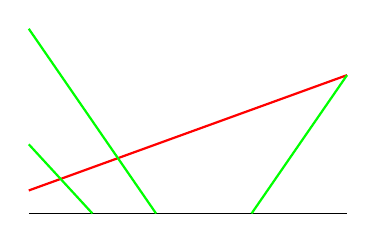
\begin{tikzpicture}[x=23,y=25]
     \draw (0,0)--(5,0) node(xline) {} ;
     \draw[red, thick] (0,0.333)--(5,2);
     \draw[green,thick] (1,0)--(0,1);
     \draw[green,thick] (2,0)--(0,2.67);
     \draw[green,thick] (3.5,0)--(5,2);
     \coordinate (p-1) at (0,4);
     \coordinate (p1) at (1,2);
     \coordinate (p3) at (2,1);
     \coordinate (p5) at (3.5,1.5);
     \coordinate (p7) at (5,4);
     \fxy{{0,...,6}}
  \end{tikzpicture}
\end{center}
In the figure the red line represents $X_c$ and the green lines the other slope variables.

\subsection{forces}
Because there are more variables than constraints
the set of variables can be devided in Free and Dependant variables.
There is always an optimal solution where the free variables are at a breakpoint.

The left-hand derivative is
\[
   \left. \frac{\partial C} {\partial x_i} \right|_- =
   \left. \frac{d f_i} {d x_i} \right|_-
   + \sum_{j \in D} \frac{\partial x_j }{\partial x_i} \frac{d f{j}} {d x_j}
\]
and the right-hand derivative is
\[
   \left. \frac{\partial C} {\partial x_i} \right|_+ =
   \left. \frac{d f_i} {d x_i} \right|_+
   + \sum_{j \in D} \frac{\partial x_j }{\partial x_i} \frac{d f{j}} {d x_j}
\]
An optimum is found if for all free variables
\[
   \left. \frac{\partial C} {\partial x_i} \right|_- \le 0 \le
   \left. \frac{\partial C} {\partial x_i} \right|_+
\]
Refer to $x_i$ as $x$, so drop the index.
The left and right derivative both have an indirect component.
It looks like a force that pushes the a breakpoint into a certain direction.
Define the force at point $x_p$ by
\[ \force(p) = - \sum_{j \in D} \frac{\partial x_j }{\partial x} \frac{d f{j}} {d x_j} \]
Around a slope the derivatives can be written as
\[
   \left. \frac{\partial C} {\partial x} \right|^{xp}_- = \plf(p-1) - \force(p)
\]
and
\[
   \left. \frac{\partial C} {\partial x} \right|^{xp}_+ =  \plf(p+1) - \force(p)
\]
At optimality we have around a point $p$
\[ \plf(p-1) \le \force(p) \le \plf(p+1) \]
If $x_p$is the lowerbound of $x$, it is the lowerbound of $x_c$ as well
\[
   \left. \frac{\partial C} {\partial x} \right|^{xp}_+ = \Dual(x_c)
      \implies \force(p) = \plf(p+1) -  \Dual(x_c)
\]
If $x_p$is the upperbound of $x$, it is the upperbound of $x_c$ as well
\[
   \left. \frac{\partial C} {\partial x} \right|^{xp}_- = \Dual(x_c)
      \implies \force(p) = \plf(p-1) -  \Dual(x_c)
\]
For breakpoint $p>c$
\[
   \left. \frac{\partial C} {\partial x} \right|^{xp}_+ = \Dual(x_{p+1})
      \implies \force(p) = \plf(p+1) -  \Dual(x_{p+1})
\]
For a breakpoint $p<c$
\[
   \left. \frac{\partial C} {\partial x} \right|^{xp}_= = \Dual(x_{p-1})
      \implies \force(p) = \plf(p-1) +  \Dual(x_{p-1})
\]

degeneracy\\
force beter indirect derivative\\
\end{document}
